% LaTeX file for resume 
% This file uses the resume document class (res.cls)

\documentclass{article} 
% the margin option causes section titles to appear to the left of body text 
\textwidth=5.2in % increase textwidth to get smaller right margin
%\usepackage{helvetica} % uses helvetica postscript font (download helvetica.sty)
%\usepackage{newcent}   % uses new century schoolbook postscript font 
\usepackage{url}
\usepackage{hyperref}
\hypersetup{
  % colorlinks,
  final,
  pdftitle={Equivariant Dendroidal Segal Spaces},
  pdfauthor={Bonventre, P. and Pereira, L. A.},
  % pdfsubject={Your subject here},
  % pdfkeywords={keyword1, keyword2},
  linktoc=page
}

\usepackage{xr}
\externaldocument{EqSegSp&G-infty-ops}

\input{commands.tex}%

%-------- TIKZ -----------------------------------------
\usepackage{tikz}%
\usetikzlibrary{matrix,arrows,decorations.pathmorphing,
cd,patterns,calc}
\tikzset{%
  treenode/.style = {shape=rectangle, rounded corners,%
                     draw, align=center,%
                     top color=white, bottom color=blue!20},%
  root/.style     = {treenode, font=\Large, bottom color=red!30},%
  env/.style      = {treenode, font=\ttfamily\normalsize},%
  dummy/.style    = {circle,draw,inner sep=0pt,minimum size=2mm}%
}%

\usetikzlibrary[decorations.pathreplacing]
% \usetikzlibrary{external}\tikzexternalize
% \makeatletters
% \renewcommand{\todo}[2][]{\tikzexternaldisable\@todo[#1]{#2}\tikzexternalenable}

% \makeatother

\begin{document} 
 
\title{Edits to ``Equivariant dendroidal Segal spaces and $G$-$\infty$-operads'' (version 3)
\\[12pt]} % the \\[12pt] adds a blank line after name
 
\author{Bonventre, P. and Pereira, L. A.}
 
\maketitle
 
The referee's preliminary report had two main sections:
first, they highlighted two specific locations for edits, % of great narrative difficulty,
and second, they offered a numbered list of recommendations and suggestions.
We have implemented the vast majority of the changes recommended by the referee, and modified the discussion around several points of confusion.
The updates are organized into four classes:
\begin{itemize}
\item in ``Requested Revisions'', we address the two unnumbered concerns of the referee.
\item in ``Comments and departures'', we answer questions posed by the referee, and indicate where and why we departed from the suggestions of the referee.
\item in ``Changes'', we address suggestions which required more significant edits to the article, or small changes regarding errors which had inhibited mathematical understanding. These changes have themselves been grouped thematically.
\item in ``Minor changes'', we list typos and other small corrections made in response to errors which did not appear to affect the referee's understanding.
\end{itemize}

Our updates are numbered by the corresponding numbered item in the referee report,
and all internal references have been modified to mathc the new numbering from the updated article.



\section{Requested revisions}

% The two locations which caused the referee confusion have been been updated.

\begin{itemize}
\item The first location, at the beginning of Section 5.2, was an unfortunate typo: %, if a maximally confusing one:
      in \eqref{OTIMESOC_EQ}, $\otimes_{\Omega[C]}$ has been changed to $\coprod_{\Omega[C]}$.
      We have also added context by recalling a similar decomposition of the product of 1-simplexes.

\item The second concerned the category $K \ltimes \mathbb R$, found in the Appendix.
      We have clarified the definition of this category in the discussion after Remark \ref{GINJ REM},
      by providing an intuitive description, a precise definition, and two examples.
\end{itemize}

      

\section{Comments and departures} % Departures from suggestions/direct answer to comments

\begin{itemize}
\item[4.] We are firmly convinced that the definitions of node, stump and root from \cite[Defs. 5.7 and 5.9]{Per18}
are correct as stated. For example, consider the tree
\begin{equation}\label{FIRSTTREE2 EQ}
	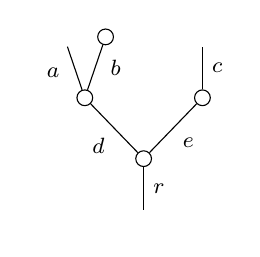
\begin{tikzpicture}[auto,grow=up,
	level distance = 2.2em,
	every node/.style={font=\footnotesize,minimum size=1.5mm}]%
	\tikzstyle{level 2}=[sibling distance=4.25em]%
	\tikzstyle{level 3}=[sibling distance=1.5em]%
		\node at (0,0)[font=\normalsize]{}%
			child{node [dummy] {}%
				child{node [dummy] {}%
					child{node {}%
					edge from parent node [swap] {$c$}}%
				edge from parent node [swap] {$e$}}%
				child{node [dummy] {}%
					child{node[dummy] {}%
					edge from parent node [very near end,swap] {$b$}}%
					child{node {}%
					edge from parent node [very near end] {$\phantom{b}a$}}%
				edge from parent node {$d$}}%
			edge from parent node [swap] {$r$}};%
	\end{tikzpicture}%
\end{equation}
The tuples $\underline{e}$ such that $\underline{e} < r$
are $de, dc, abe, abc, ae, ac$, and $r^{\uparrow} = de$ is the maximum of these.

We are also unsure of how replacing ``maximum'' with ``upper bound'' would change these definitions, since an upper bound of a subset $A$ that is also in $A$ is automatically the maximum of $A$.  %

\item[5.] All instances of minimal/maximal/smallest/etc were checked, and we believe they were correct as stated. A few instances were the article ``the'' was meant to convey uniqueness (i.e. ``the minimal/maximal'') were altered to reduce the potential for misunderstanding (to ``the smallest/largest''). %

\item[9.] Rephrased the language in the proof of Lemma \ref{CUPCAP LEM} to explain why the argument isn't circular. The main point comes down to the fact that ``edge'' and ``vertex'' are simply suggestive names for ``element'' and ``generating relation'' of the broad poset. %
      
\item[24.] Clarified the definition of ``built cellularly'' from Lemma \ref{CHAREDGE LEM}, and added references for related terminology. %
      % (in particular, distinguished it from the class of saturated maps)
      % Reworded ``is cellular on'' to ``is built by attaching'' $G$-inner horn inclusions


\item[25.] Added a reference to Goodwillie for the use of the adjective ``convex'' before the proof of Lemma \ref{CHAREDGE LEM}, and included the name ``downward closed''.
      As our argument is similar in spirit to that of Goodwillie's, we have chosen to continue using his nomenclature. %

      
\item[27.] At the end of the proof of Lemma \ref{CHAREDGE LEM}, the new (Ch2) follows from the original conditions, but it requires both the original (Ch2) and (Ch3), which work in tandem. The discussion was expanded to provide more detail on this point. %
      
      As a side note, (Ch2) and (Ch3) are complementary, and if it weren't for the fact that equivariance forces us to worry about isotropies, I believe they could be combined without much worry.
      However, separating (Ch3) is needed to control the isotropies (which is why (Ch3) is needed when verifying condition (c) in the proof). In fact, in earlier iterations of the characteristic edge lemma condition (Ch3) used to make explicit reference to elements $g \in G$, before the current version of (Ch0) was identified. %
     

\item[37.] I do not think the proof of Proposition \ref{HYPER PROP} should require anything analogous to the mentioned condition (b) in the proof of Lemma \ref{CHAREDGE LEM}.
      The main idea is that for $U \in \Omega$ and $V \hookrightarrow$ a planar face, it is $|V|<|U|$ unless $V=U$. We've added an extra sentence to Remark \ref{FACCES REM} to clarify this point. % that should make this point clearer. %
      

\item[53.] The adjunctions from this notation are only used in a single instance, in the proof of part (i) of Proposition \ref{SSSETJREE PROP}; moreover this use is also simpler since only the single $\partial \Delta[m]$ isn't a representable.
      Because of this, it feels somewhat unnecessary to fully expand on the adjunctions at this point in the discussion,
      rather than wait until (the new) Remark \ref{TWOVARADJ REM}. %

\item[56.] Added the new Remark \ref{TWOVARADJ REM} discussing the two-variable adjunction and associated lifting properties. %

      


\end{itemize}



\section{Changes}

\begin{itemize}

      % --------- OUTER/ORBITAL FACES ----------
      \subsubsection*{Orbital faces and outer closures}
\item[8.] Clarified the definition of ``outer face map'' and corrected ``non-identity'' to be ``non-isomorphism'', before Proposition \ref{UNIQUEFACT PROP}.%
      
\item[11.] Converted the previous ``factorization of orbital faces'' remark into Proposition \ref{INNOUTORB PROP} and proved it.
      
Edited Proposition \ref{UNIQUEFACT PROP} to also include a statement about planar maps.

Expanded Notation \ref{BARUT NOT} when defining ``outer closure'' in to clarify both its meaning and why such an outer face exists. %

\item[12.] Reworded Proposition \ref{MINGFACT PROP} to state that $GU$ is the smallest orbital face containing $U$.
      
      Changed the language in the proof to reflect the restatement and provide some extra detail. %
      
\item[13.] The ``$\leq_d$-incomparability of components'' language was removed from the proof of Proposition \ref{MINGFACT PROP} in favor of a better explanation for Remark \ref{ROOTISOMONO REM} from Point 15 below (which was moved to before this result) %
      
\item[14.] Reworded the ending of the proof of Proposition \ref{MINGFACT PROP} to clarify the argument and be consistent with the rewording of the proposition itself. %
      
\item[15.] The remark concerning when $G\cdot_H U \to T$ is injective was moved to an earlier point, Remark \ref{ROOTISOMONO REM}, and a clearer explanation was provided. %

\item[23.] Adapted the definition of outer closure from Notation \ref{BARUT NOT} to also include non-planar faces.
      
\item[34.] Adapted the definition of $GV$ from Proposition \ref{MINGFACT PROP} to also include non-planar faces.
      



      % ---------- CHAREDGE LEM ----------
      \subsubsection*{Characteristic edge lemma}
\item[26.] Added a new paragraph to the proof of Lemma \ref{CHAREDGE LEM} explaining why conditions (a)(b)(c) imply that the square \eqref{FIRPUSH EQ} is a pushout. %

\item Added a little more detail to the discussion of Example \ref{THM71 EX} to better explain the role of elementary trees.

\item[30.] Corrected $A_C = 
      A \cup \bigcup_{g\in G,V \in C} g b_{[e]}(\Omega[V])$ in the final paragraph of Remark \ref{CHAREDGE2 REM}.
      
      Similarly, added the alternate $g \Omega[V]$ formula already in the proof of the characteristic edge lemma.
      
      Moreover, expanded Remark \ref{FACEGACT REM} to explain why $\Omega[gV] = g\Omega[V]$ and better explain the connection with isotropy of representable subpresheaves. %
      

      
            
      % ---------- hypersaturations ----------
      \subsubsection*{Hypersaturations}
\item[39.] In the proof of Proposition \ref{HYPER PROP},
      the given argument for the Segal hypersaturation indeed used $T \in \Omega^G$. Since this made the discussion somewhat awkward, we've moved the argument being made to (the new) Proposition \ref{SCANOD PROP}, and rephrased accordingly. %
      
\item[42.] Clarified the meaning of hypersaturation in the paragraph before Proposition \ref{HYPERLP PROP} when not assuming that the maps are cofibrations. %

\item Added Remark \ref{DUMBHYPER REM} to clarify a hypersaturation argument used repeatedly in the paper.      

      

      
      % ---------- normal monos ----------
      \subsubsection*{Normal monomorphisms}      
      
\item[21.] Provided references for the characterization of $G$-normal monomorphisms in the paragraph after Remark \ref{FACEGACT REM}. %   
      
\item[69.] Reworded the proof of Lemma \ref{GENSET LEM} describing the normal generators of $\mathsf{PreOp}^G$ to avoid the confusing wording. %

\item[70.] Completed the proof of Lemma \ref{GENSET LEM} by indicating why the generators are normal. %   
 


      

      % ---------- fibrant objects ----------
      \subsubsection*{Joint localizations and characterizations of fibrant objects}
\item[1.] Added the names of the fibrant objects to the introduction when naming the model structures in question, as well as included a version of the table produced by the referee (and references to the categorical narrative).
      
\item[2.] Added Remark \ref{RECOVDEF REM} which explains why our results extend \cite[Thm. 6.6]{CM13a} and clarified the influence of \cite[Thm. 6.6]{CM13a} in the introduction (to the paper and to \S 4). %
      
      % ---------- JOINTFIBCHAR PROP ----------
\item[62.] The confusing wording in the proof of Proposition \ref{JOINTFIBCHAR PROP} has been changed (the reason for the wording was the fact that I was trying to point out that the condition in the (new) \ref{HYPERMODEL REM} had to be checked).
      
      Added reference to Remark \ref{HYPERMODEL REM} in Proposition \ref{SSSETJREE PROP} and in Remark \ref{HYPERSIMPL REM}.
      
\item[63.] Edited proof of Proposition \ref{JOINTFIBCHAR PROP} to explain why the given condition shows $X_L,X_k $ are fibrant.
      
\item[64.] Edited proof of Proposition \ref{JOINTFIBCHAR PROP} to explain why the maps $\Omega[T] \otimes (\{i\} \to J)$ suffice. %
      
\item[65.] As written, Corollary \ref{REGGENHORN COR} was indeed needed to finish the argument in Proposition \ref{JOINTFIBCHAR PROP} (which was previously called a Corollary). This has been addressed by adding the generating horn inclusions $\Lambda^{Ge}[T] \to \Omega[T]$ to Proposition \ref{HYPER PROP}. %
      % ----------
      
\item[67.] added Definition \ref{SEGALOP_DEF} defining equivariant Segal operads after the proof of the model structure on $\mathsf{PreOp}^G$, Theorem \ref{PREOPMOD THM},
      
      Added Remark \ref{SEGALOP_REM} concerning the fibrant objects being the Reedy fibrant Segal operads. %
      % as fibrant objects
      %% the Segal operads are not exactly the fibrant objects. It is convenient to have a larger class. This is used in the third paper once tame model structures enter the picture, since the tame fibrant stuff still satisfies the Segal operad condition, despite not being dendroidal Reedy fibrant
      
\item[74.] Added Proposition \ref{DSSCHAR_PROP} to the beginning of \S 5.1 characterizing equivariant dendroidal Segal spaces in the vein of \cite[Cor. 5.6]{CM13a}. %



      
      % ---------- ho(X) ----------
      \subsubsection*{The homotopy genuine equivariant operad}
\item[76.] Turned the claim that $ho(X)$ is a genuine equivariant operad into the new Proposition \ref{HMTPYGEN PROP}, and gave a full proof.
      
      % added the actual formulas for $X(A)$, since they get used here...
      
      Added an alternate formula for $\upsilon_{\**}$ after \eqref{DSETG_EQ}.
      
      Added Remark \ref{UPSPUSHMON REM} noting that $\upsilon_{\**}$ preserves certain pushouts %
      
      % added internal references which show that $ho(X)$ is a genuine equivariant operad
      
\item[78.] Corrected and clarifed the equation in Definition \ref{HMTPYGEN DEF} describing the coefficient system of categories part of the homotopy genuine operad. %

      
      
      
      % ---------- J STUFF ----------
      \subsubsection*{The simplicial set $J$}
\item fixed typo in Remark \ref{CONTGR REM} stating that $N[m] \to N \widetilde{[m]}$ is built from $0$-horns. Namely, ``$m$-simplex $\underline{a}$'' should have been ``$k$-simplex $\underline{a}$'' %

\item[66.] Edited Notation \ref{JM NOT} defining $J^m$ to provide a little more information.

Added the new Remark \ref{JREEDYCOF REM} immediately after said notation proving that $J^{\bullet}$ is Reedy cofibrant cosimplicial.

Added reference to this new remark in the discussion in Remark \ref{CONCRECOM REM}.

Added reference to this new remark in the proof of Proposition \ref{COMPLE PROP}.

Added a definition of the bisimplicial $X(-)$ notation immediately before Proposition \ref{SESP PROP}.

Edited Proposition \ref{SESP PROP} and its proof to replace appearances of $n$ with $m$. %

\item[72.] Added explanation in Lemma \ref{TRIVFIB LEM} for why $X \otimes J$ is a cylinder object. %

\item[81.] Added an explanation to Proposition \ref{SESP PROP} for why $X^h(J) = X(J)$. %     

      Slightly strengthened Proposition \ref{SESP PROP}(iv) to include weak equivalences $X(J^m) \to X^h(m)$ for all $m$ (to be used in the revised proof of Proposition \ref{COMPLE PROP}).

      
      
      % ---------- Section 5.2 ----------
      \subsubsection*{Edits for \S 5.2}
\item Expanded the discussion of cube fibrancy/cofibrancy before and during the proof of Proposition \ref{JDDK PROP}, and (hopefully) made the overall argument a little clearer. %
      
\item Added reference for why $X^{\Omega[T]}$ is Segal space in Proposition \ref{JDDK PROP}. %

\item Fixed the incorrect $\iota^{\**}_G$ notation issue at the end of the proof of Proposition \ref{JDDK PROP} by circumventing that notation. %
      
\item Added Remark \ref{DKCOM REM} (which may become a proposition...) which performs the argument about DK equivalences inducing equivalences on fibers
      
      Added Corollary \ref{DKCOM COR} that spells out some key consequences of \eqref{DKCOM REM}

      
\item[55.] Rewrote the proof of and improved Corollary \ref{SSETSSETADJ COR} to add a sufficient condition for when $\delta^{\**}(X)$ is a Kan complex (to be used in the revised proof of Proposition \ref{COMPLE PROP}), and expanded the succeeding Remark \ref{HYPERSIMPL REM} to reflect this.
      
      % A Large portion of this proof has been rewritten with some slight changes in notation and more details provided, including fixing the math typo where $G$ should have been $\Lambda^i[n] \times G$.

      
\item Major rewrite of the proof of Proposition \ref{COMPLE PROP}.
      
      Added Remark \ref{LAMBJREAL REM}, which does a quick argument needed for the proof of the revised proof of Proposition \ref{COMPLE PROP}.

      Added Remark \ref{COMPLE REM}, commenting on how the proof of Proposition \ref{COMPLE PROP} now is a little different from the analogous proposition in \cite{Rez01}.

\item Simplified the notation in the proof of Theorem \ref{COMPIFFDK THM} to simplicial Segal space notation, since now the dendroidal part of the story has already been taken care of elsewhere. Also added a little extra detail to the arguments.

\item Fixed the formula for $(\mathsf{csk}_{\eta} Y)(B)$ in Proposition \ref{CSKETALT PROP}, which was missing the $G$-fixed points.
      
      
      % ---------- Appendix ----------
      \subsubsection*{Edits to the appendix}
\item[58.] A brief discussion of cofibrant generation for Reedy model structures was added to the end of the appendix, in particular Proposition \ref{REEDYCOFGEN PROP}. The proof of this result, Proposition \ref{SDSETJRCOF PROP} was reworded accordingly. %
      
\item Added short proof to Proposition \ref{FGTRL_PROP}. %


      

      % ---------- incorrect references ----------
      \subsubsection*{Incorrect references}
      
\item[6.] Fixed reference \cite[Prop. 3.21]{BP17} to \cite[Prop. 3.23]{BP17}, and clarified the citation for \cite{BP17}.

\item[48.] Fixed reference \cite[Prop. 3.4.18]{Hir03} to be \cite[Thm. 3.3.18]{Hir03} (I had an old version of the paper).
      
      In addition, some extra detail concerning how \cite[Prop. 3.3.18]{Hir03} was being used was added, and some of the notation in Proposition 4.1 and its proof was adjusted to allow for this.
      
      In further addition, made an observation as to why cofibrant approximation is a non issue.
      
\item[49.] Fixed reference to \cite[Thm. 3.3.8]{Hir03} to be \cite[Thm. 3.2.13]{Hir03} (I had an old version of the paper)
      
\item[85.] Modified the reference \cite[\S 4]{BM11} to \cite[\S 4,\S 6]{BM11}, to note that \S 6 is where (co)skeleta are actually discussed.
      
\item updated the reference to ``Equivariant Dendroidal Sets'' and other articles to reflect their publication,
      and checked all references to these papers to ensure that they match the final version. %




      % ---------- notation ----------
      \subsubsection*{Notation}
\item[41.] Added Notation \ref{DELTAOMEGA NOT} to the end of \S 2.1 comparing $\Omega$ to $\mathsf{sSet}$, and introduced the stick tree $\eta$. %

      
\item[43.] Clarified in Remark \ref{NORMMAP REM} that the ``single colored $G$-operad'' is on the category of sets. %

      
\item[44.] Added comment to Remark \ref{NORMMAP REM} that $\Omega(T)$ is the operad generated by $T$ and added references. %

      In addition, included the $\Omega(T)$ notation and references in the first paragraph of \S 2.1 when the similarity between the broad poset and the operad generated by $T$ is mentioned. %

      
\item[68.] Explained the $\mathsf{csk}_{\eta}$ notation in the paragraph before Proposition \ref{CSKETALT PROP}. %     
      

                           
\end{itemize}








\section{Minor changes}
 
% The following lists the corrections of typos and other smaller mistakes listed in the preliminary referee report.

\begin{itemize}
\item[3.] added missing relation $aef \leq r$ to ``The other broad relations obtained by broad transitivity are \dots''
\item[7.] added ``$\varphi$''
\item[10.] reworded to ``denote the category of $G$-objects''
\item[16.] fixed ``of a leaf'' typo
\item[17.] changed ``does not act'' to ``acts trivially''
\item[18.] Deleted ``In fact''
\item[19.] Rephrased the $T/G$ remark to mention at the beginning that $T/G$ is formally defined below.
\item[20.] Replaced ``is an orbital $G$-subset'' with ``is a transitive $G$-subset''
\item[22.] added ``$\emptyset \neq E$''
\item[28.] explained what ``associative and unital'' means for the isomorphisms $U_i \xrightarrow{g} U_{gi}$
\item[29.] replaced instances of $Y$ with $B$
\item[31.] replaced ``subsets'' with ``simplicial subsets'' in the discussion of covers (``which in our language are the simplicial subsets'')
\item[32.] added comment noting that the ``dendroidal cover'' definition extends to the equivariant context
\item[33.] added the missing word ``planar'' to ``$G$-poset of outer faces''
\item[35.] added comment saying that in the proof of the second ``anodyne horn inclusion'' lemma we again assume $T \in \Omega^G \subseteq \Omega_G$.
\item[36.] reworded the definition of hypersaturated class
\item[38.] fixed $\Lambda^EF[T]$ typo
\item[40.] changed the $T$'s to $S$'s in Remark \ref{ORBHYPER_REM} % containing \eqref{ORBHORNPUSH EQ}
%%% When rereading I noticed that I had followed this convention in Corollary REGGENHORN COR, so this is a preferable fix for consistency
%this is a matter of taste, but I find changing $T$ to $S$ in $\Lambda^E_o[T] \to \Omega[T]$ to contrast with $Sc[T] \to \Omega[T]$ to be a bit confusing. To emphasize that both of the $T$ variables are free, rather than chosen, I've instead added ``$T\in \Omega_G$'' to both expressions.
\item[45.] Changed ``Theorem 6.1'' to ``Thm. 6.1'' when citing MW09 (in the Remark discussing why strict lifting properties in $\mathsf{dSet}^G$ are unsatisfactory)
\item[46.] changed ``genuine'' and ``na\"ive'' to ``fine'' and ``coarse''.
\item[47.] Added missing dot to ``Thm. 2.1'' in the citation from Per17 (at the beggining of \S 4)
\item[50.] added comment saying that ``$\square$ denotes the pushout product''
\item[51.] added $n \geq 1$ condition
\item[52.] added $m \geq 1$ condition
\item[54.] fixed ``monormorphism'' typo
\item[57.] added $n \geq 1$ condition
\item[59.] clarified that it is the ``simplicial structure maps $X_0 \to X_n$'' that need to be weak equivalences
\item[60.] replaced ``equivalences in $\mathsf{dSet}^G$'' by ``weak equivalences in $\mathsf{dSet}^G$'' in part (ii) of the Corollary
\item[61.] clarified that it is the ``natural maps'' that need to be Kan equivalences
\item[71.] added ``normal'' to ``a map $X\to Y$ in $\mathsf{PreOp}^G$ will have the right lifting property against all monomorphisms''
\item[73.] fixed $\mathsf{Preop}^G$ typo
\item[75.] fixed $x_n$ instead of $x_k$ typos
\item[77.] Recalled that $\mathsf{O}_G$ is the orbit category.

Similarly, a similar comment was added in the remark immediately preceding \S 4.
\item[79.] fixed $\varphi$ to be $\psi$
\item[80.] changed the $H$-equivalence from ``$f$'' to ``$j$'' to avoid confusion
\item[82.] fixed ``automorphim'' typo
\item[83.] removed the word ``degeneracy'' in the discussion of generalized Reedy category structure on $G \times \mathbb{S}$
\item[84.] added comment saying that ``$L_r$ and $M_r$ are recalled below'' before the theorem
\item[86.] changed ``genuine'' to ``fine''
\item[87.] Fixed the indexes in the ``extension of partial factorizations'' lemma
\end{itemize}



\bibliography{biblio}{}

\bibliographystyle{alpha}


\end{document} 




%%% Local Variables:
%%% mode: latex
%%% TeX-master: t
%%% End:
